% ПЛАН

%# Глава 1 – Алгоритмы оценки параметров гармоник и их применение для многотональных сигналов.
%
%Выводы по главе: 
%- Особенности сигналов в электрических сетях носят не существенный характер с точки зрения построения алгоритмов нахождения параметров гармоник. При работе с электрическими сетями обычно используют стандартные алгоритмы такого рода.

%- Помимо обычных алгоритмов для оценки параметров гармоник в электрических сетях также используют алгоритмы, анализирующие сигналы в переходных режимах, т.е. такие, в которых во время работы алгоритма может измениться значение какого-либо параметра. В нашей работе такие алгоритмы далее рассматриваться не будут, поскольку переходные режимы не являются целью нашей работы.

%- Анализ имеющихся библиографических источников показывает, что нет известных публикаций в которых бы велась разработка алгоритмов, ориентированных на работу при определенном соотношении сигнал-шум, и что для анализа гармоник и интергармоник (для которых это соотношение отличается) применяются одинаковые алгоритмы.

%- Алгоритмы оценки параметров гармоник, применяемые при работе с одно- и многотональными сигналами, имеют точность оценки параметров ниже теоретической границы Крамера-Рао. Вопрос о причинах снижения точности и возможности построения алгоритма, достигающего этой границы в известных научных публикациях не рассмотрен.

%- Для решения задачи построения оптимального алгоритма для анализа спектра сигнала в электрических сетях необходимо уточнение математической модели спектра сигналов в части, описывающей точность оценки (дисперсию) параметров гармоник спектра многотонального сигнала.
%
\chapter{ Алгоритмы оценки параметров гармоник и их применение для многотональных сигналов.}\label{ch:ch1}

\section{Концепция определения гармоник} \label{sec:ch1/sec1}

Нелинейная нагрузка – это нагрузка, в которой ток потребления не синусоидален при условии питания синусоидального источника напряжения.
Параметры коммутируемой нагрузки установлены в ОСТ $1 00392 - 80$  «Аппараты коммутационные. Методика определения параметров нагрузок и выбора аппаратов по параметрам коммутируемой нагрузки» от $30$   сентября $1980$~г. (дата актуализации  $01.01.2019$~г.):

\begin{itemize}
	\item номинальное напряжение $U_n$;
	
	\item максимально потребляемая сила тока $I_{ust}$;
	
	\item эквивалентная электромагнитная постоянная времени $T_{e}$;
	
	\item амплитуда импульса силы тока $I_m$;
	
	\item длительность импульса силы тока  $\varDelta t_u$;
	
	\item длительность фронта импульса силы тока $\varDelta t_f$;  (возникает в переходном режиме).
\end{itemize}

Нелинейные и коммутируемые нагрузки могут вызвать искажения нормальных синусоидальных сигналов тока и напряжения в системе переменного тока. Это искажение формы волны может характеризоваться рядом синусоидальных компонентов на гармонических частотах и синусоидальных компонентов на интергармонических частотах.
 
Спектральные составляющие, относящиеся к интергармоникам, изменяются по амплитуде и по частоте. Интергармоники – это токи или напряжение, которые не кратны основной частоте переменного тока.

Концепция гармоник основана на анализе Фурье, чтобы восстанавливать несинусоидальную периодическую форму волны по серии синусоидальных компонентов. Если $x(t)$  непрерывный периодический сигнал с периодом $T$   и удовлетворяет условию Дирихле, его можно представить в виде ряда Фурье:

\begin{equation}
	\label{eq:equation1.1}
x(t) = \displaystyle\sum_{k=\infty}^{\infty} X(k \omega_{0}) e^{jk \omega_{0} t}
\end{equation}

где $\omega_0 = \frac{2 \pi}{T}$  называется угловой частотой;
 
$X(k \omega_{0})$ является коэффициентом Фурье на $k$ – гармонике.  

Коэффициент Фурье определяется как:
\begin{equation}
\label{eq:equation1.2}
X(k \omega_{0}) =  \frac{1}{T} \int_t^{t+T} x(t) e^{-jk \omega_{0} t} {d}t
\end{equation}

Несинусоидальный периодический сигнал может быть разделен на ряд синусоидальных компонентов с частотами, которые являются целыми, кратными основной частоте. Для ряда Фурье сигналы имеют бесконечную длину, во временной и в частотной области.
Для нахождения ряда Фурье применяют цифровые методы, то есть алгоритм дискретного преобразования Фурье (ДПФ, DFT – Discrete Fourier Transform) или его вариант – быстрое преобразование Фурье (БПФ, FFT – Fast Fourier Transform). Для этого анализируемый аналоговый сигнал подают на вход аналогово-цифрового преобразователя. Полученные отсчеты запоминают. Каждая группа из  отсчетов соответствует временному интервалу измерения, в котором осуществляется ДПФ.
Предположим, что $x(t)$ отбирается со скоростью $N$  точек в течение цикла, $T_s =\frac{T}{N}$. ДПФ определяется как:

\begin{equation}
	\label{eq:equation1.3}
(\omega_{k}) =  \displaystyle\sum_{n=0}^{N-1} x(n) e^{-j \frac{2 \pi}{N}nk}, k = 0,1, ..., N-1
\end{equation}

где $\omega_{k} = \frac{2 \pi}{T_s N} k = \frac{2 \pi}{T} k$

$X (\omega_{k})$ -- это спектр $x(n)$.
 
Предполагаем, что $x(n)$  – это один цикл периодического сигнала. То есть, сигнал должен точно повторяться для каждой   точек.

Угловое разрешение по частоте спектра определяется длиной сигнала как:

\begin{equation}
	\label{eq:equation1.4}
\bigtriangleup \omega = \frac{2 \pi}{T}
\end{equation}

Спектр сигнала состоит из комплексных чисел. В комплексном виде закодированы амплитуда и угол. Амплитуда является количественной характеристикой синусоидального сигнала. Угол позволяет увидеть смещение по фазе.

Таким образом, если $T$ выбран в качестве одного из периодов $x(n)$, спектр результатов будет показывать только компоненты, которые являются кратными основной частоте и определены как гармоники. Если длина данных выбрана как  $N$ циклов ($N>1$ , целое число), то основное разрешение по частоте будет меняться как:

\begin{equation}
	\label{eq:equation1.5}
\bigtriangleup \omega = \frac{2 \pi}{NT} = \frac{\omega_1}{N}
\end{equation}

Это подразумевает, что можно использовать более одного основного цикла для выполнения ДПФ. Становится возможным получать компоненты на частотах, которые не кратны основной частоте. Эти компоненты нецелого порядка, в соответствии с определением  Международной электротехнической комиссии (МЭК, IEC -- International Electrotechnical Commission) называются интергармониками. Например, если выбрать пять циклов по $60$~Гц для преобразования Фурье, разрешение по частоте будет $\bigtriangleup f = \frac{60}{5} = 12$~Гц, тогда можно получить отсчеты (бины) на частотах $12$~Гц, $24$~Гц, $36$~Гц,... Эти компоненты, определяются как интергармоники.

Для оценки гармоник результаты ДПФ должны быть сгруппированы, чтобы получить сумму квадратов значений промежуточных спектральных составляющих между двумя смежными гармониками в соответствии с выражением \cite{GOST30804.4.7-2013}: 
% Внести источник
 
\begin{equation}
	\label{eq:equation1.6}
Y_{(g,h)}^2 = \frac{1}{2} Y_{C,(Nh)-\frac{N}{2}}^2 +  \displaystyle\sum_{k=(-\frac{N}{2})+1}^{\frac{N}{2}-1} Y_{C,(Nh)+k}^2 + \frac{1}{2} Y_{C,(Nh)+\frac{N}{2}}^2
\end{equation} 
 
где $Y_{C,(Nh)+\frac{N}{2}}^2$  – среднеквадратичное значение спектральной составляющей (соответствует конкретной частотной позиции ДПФ);

$(Nh) + k$ – номер спектральной составляющей;

$Y_{(g,h)}$ –   среднеквадратичное значение гармонической группы (r.~m.~s. value of a harmonic group).

Индекс $C$ предназначен для отнесения переменных к спектральным составляющим.

Должно проводиться сглаживание среднеквадратичных значений $Y_{(g,h)}$ каждого гармонического порядка, рассчитанного по формуле \ref{eq:equation1.6}, с использованием цифрового эквивалента фильтра низких частот $1$-го порядка с постоянной времени  $1,5$~c.
% Проверить формулу 6.

В гармонической группе суммируется энергия ближайших спектральных составляющих с энергией гармоники. Порядок гармонической группы определяется порядком рассматриваемой гармоники. Среднеквадратичное значение интергармонической группы (r.~m.~s. value of an interharmonic group) между гармониками порядка $h$ и $h+1$ обозначают $Y_{(ig,h)}$.

При использовании группирования учитывают все спектральные составляющие, а не только спектральные линии на частотах, кратных основной частоте (гармоники). Группирование спектральных составляющих в интервале частот между последовательными гармоническими составляющими образует интергармоническую группу. Это группирование позволяет учесть значения спектральных составляющих, возникающих между двумя последовательными гармониками, а также учесть результаты флуктуации напряжения (фликер). Процесс образования гармонических и интергармонических подгрупп напряжения схематично представлен на \ref{img:picture1.1}.
Спектральные составляющие, которые относятся к интергармоникам, изменяются по амплитуде и частоте. Группирование спектральных составляющих в интервале частот между последовательными гармоническими составляющими образует интергармоническую группу. Это позволяет учесть значение спектральных составляющих, возникающих между двумя последовательными гармониками.

\begin{equation}
	\label{eq:equation1.7}
	Y_{ig,h}^2 = \displaystyle\sum_{k=1}^{N-1} Y_{C,(N \cdot h)+k}^2 
\end{equation}  

где $Y_{ig,h}^2$ – среднеквадратичное значение интергармонической группы (r.~m.~s. value of an interharmonic group);

$Y_{C,k}$ – среднеквадратичное значение спектральной составляющей, порядка;

$h$ – целое число, обозначающее порядок гармоники;

$k$ – целое число, обозначающее порядок спектральной составляющей;

$C$ – значение относящееся, к спектральным составляющим. 

Особенность анализа с использованием алгоритмов ДПФ заключается в том, что необходимо обрабатывать данные сигнала из одного периода. При обработке данных выполняется периодическое расширение сигнала, с использованием ДПФ. Между последовательностями получаются разрывы. Отсюда следует, что возникают спектральные искажения, которые отсутствуют в исходном сигнале. Явление называется просачиванием спектральных составляющих. Поэтому появляются сигналы, которых нет на входе. Для уменьшения таких влияний перед вычислением ДПФ, умножаем отчеты на весовую функцию. 

Существуют различные весовые функции: Прямоугольное окно (Rectangle window), окно Барлетта (Bartlett window) или треугольное окно, окно Ханна (Hann window), окно Барлетта-Ханна (Bartlett–Hann window), окно Хемминга (Hamming window), окно Гаусса (Gaussian window) и другие. Несвойственные интергармонических компоненты строго зависят от спектральных характеристик принятого окна. 
ДПФ и БПФ позволяют получить точные результаты только при установившихся сигналах. Сигналы, амплитуды которых изменяются во времени, не могут быть точно характеризованы только совокупностью их гармонических составляющих.

\begin{figure}[ht]
	\centering
	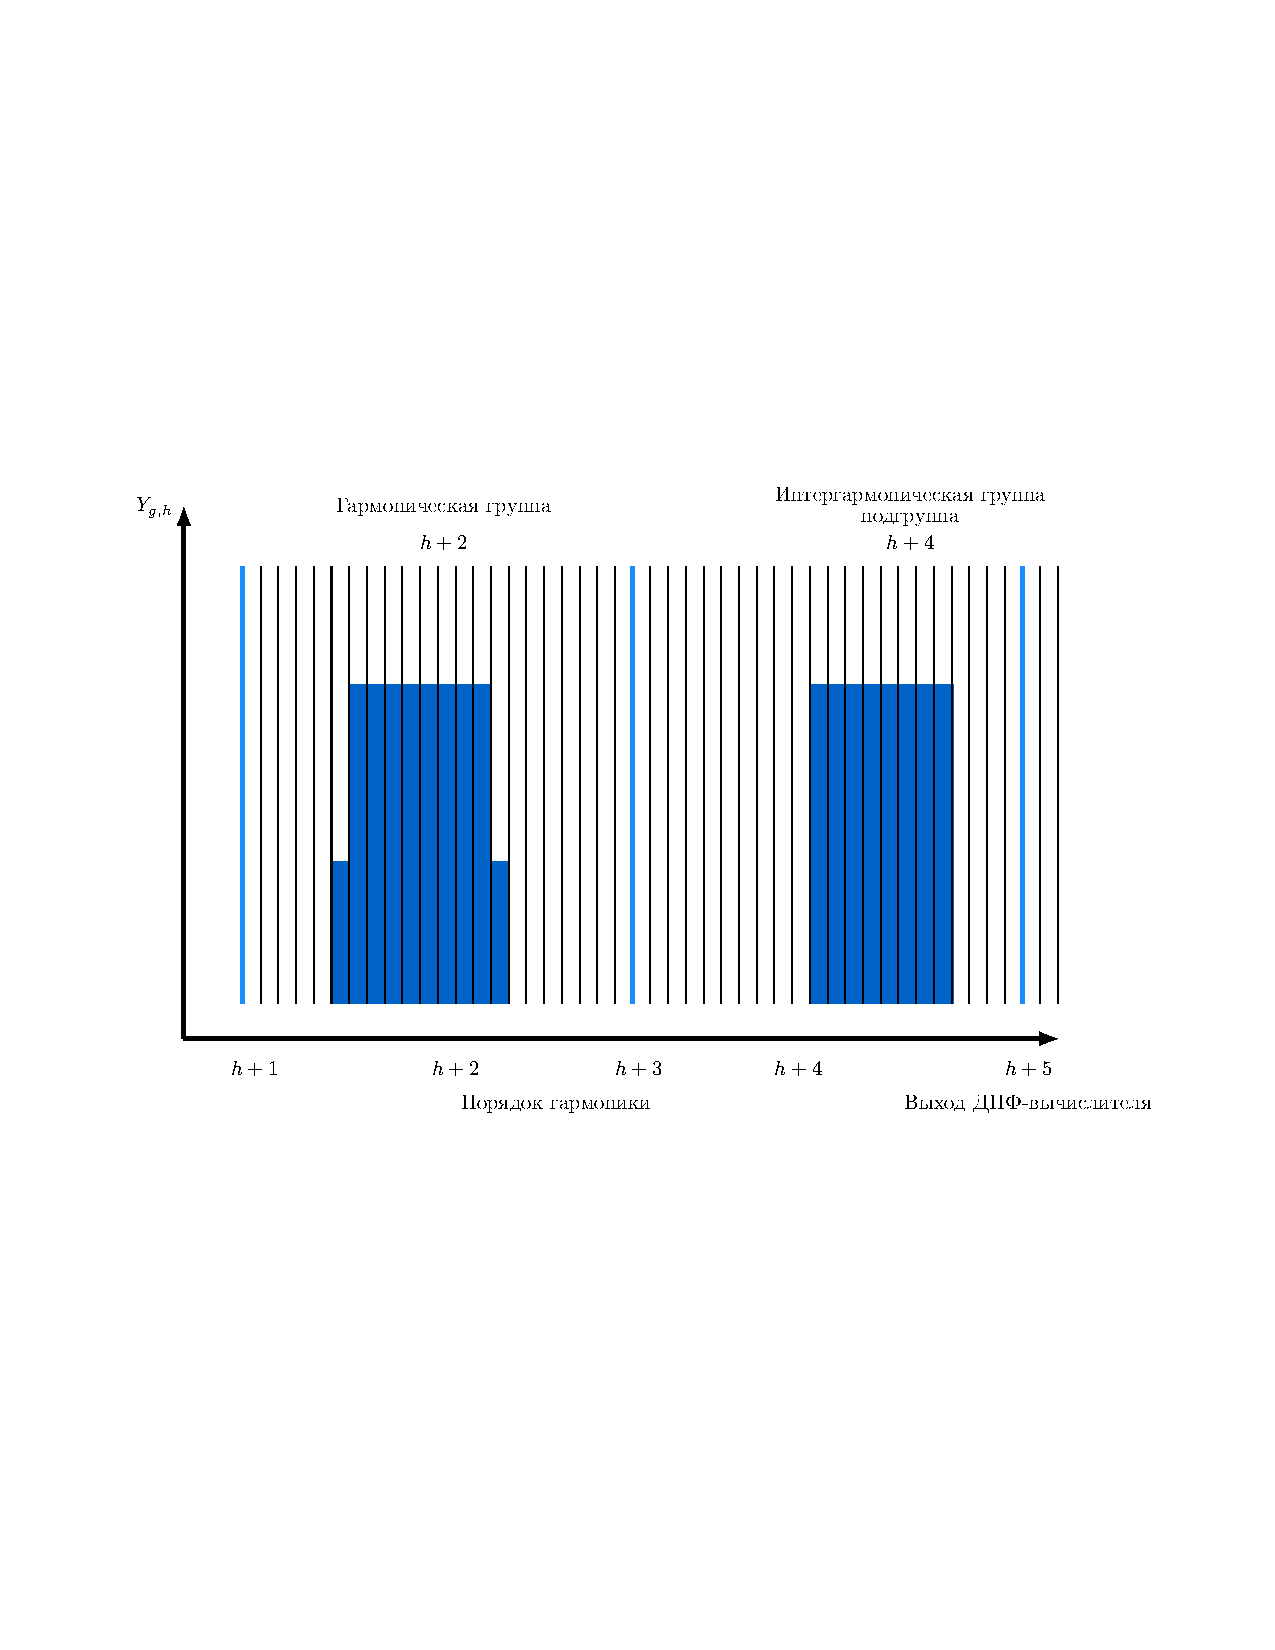
\includegraphics [scale=0.9] {scheme_of_harmonic_and_interharmonic_groups}
	\caption{Схема образования гармонических и интергармонических групп (для систем электроснабжения частотой  $50$ Гц).}
	\label{img:picture1.1}
\end{figure}

\begin{figure}[ht]
	\centering
	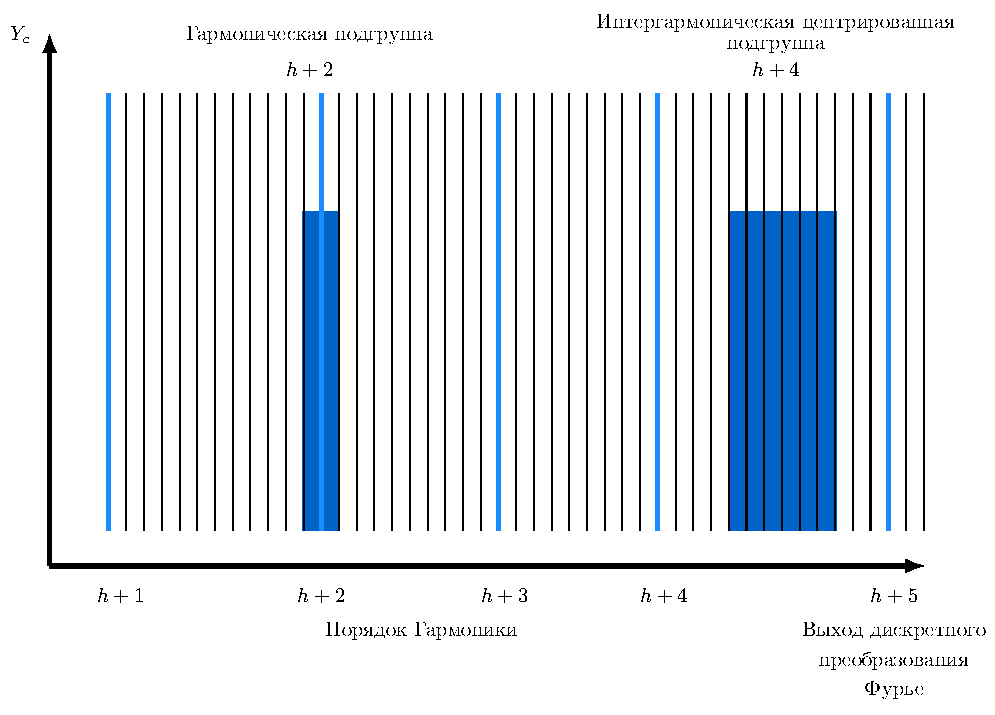
\includegraphics [scale=0.9] {process_of_harmonic_and_interharmonic_groups}
	\caption{Схема образования гармонических подгрупп и интергармонических центрированных подгрупп (для систем электроснабжения частотой  $50$ Гц).}
	\label{img:picture1.2}
\end{figure}

Примерами регулярно колеблющихся нагрузок, которые вызывают синусоидальные и квадратно-модулированные сигналы, являются сварочные аппараты, лазерные принтеры и приборы с интегральным контролем цикла. Для таких нагрузок частота, с которой изменяется нагрузка, будет определять частоты интергармоник.

Предполагая, что напряжение системы   и нагрузка имеет характеристику $R(t) = 1 - r \sin 2 \pi f_{0} t$, где $r<1$ и $f_{0}$  частота нагрузки варьируется. Тогда ток нагрузки: 

\begin{equation}
	\label{eq:equation1.8}
	i(t) = \frac{\upsilon (t)}{R (t)} = \frac{\sin 2 \pi f t}{1 - r \sin 2 \pi f_0 t} = \sin 2 \pi f (1 + r \sin 2 \pi f_0 t + r^2 \sin^2 2 \pi f_0 t + r^3 \sin^3 2 \pi f_0 t + \dots) 
\end{equation} 

Согласно \ref{eq:equation1.8}, $i(t)$  содержит компоненты интергармоник $f\pm f_{0},f\pm 2f_{0}, f\pm 3f_{0}, \cdots $ и~т.~д. Интергармоники будут представлены в текущем спектре $f_0$ асинхронно с $f$. 
Несинусоидальность напряжения, вызываемая высшими гармониками (ВГ), отрицательно влияет на работу силового электрооборудования и автоматики в системах электроснабжения. Из-за несоответствия норм коэффициента искажения синусоидальной формы кривой напряжения, возрастают потери электроэнергии. Повышается аварийность в кабельных сетях, вызывая сбой в работе систем релейной защиты, автоматики, телемеханики и связи.
Нормы показателей качества электрической энергии, относящиеся к несинусоидальности напряжений, измеряются и оцениваются с учетом влияния не только высших гармоник, но и групп близко расположенных комбинационных (интергармонических) составляющих \cite{532851}.
%Yacamini R. Power system harmonics. IV. Interharmonics //Power Engineering Journal. – 1996. – Т. 10. – №. 4. – С. 185-193.


Суммарный коэффициент гармонических составляющих (THD – total harmonic distortion) – это отношение среднеквадратичного значения суммы всех гармонических составляющих $Y_{H,h}$ до порядка $h_{max}$ к среднеквадратичному значению основной составляющей $Y_{H,1}$. 

\begin{equation}
	\label{eq:equation1.9}
THD_{Y} = \sqrt{\displaystyle\sum_{h=2}^{h_{max}}} (\frac{Y_{H,h}}{Y_{H,1}})^2
\end{equation} 
где $h_{max}=40$, если другое значение не установлено в международных стандартах, характеризующих нормы эмиссии гармоник.

Для тока используем символ $I$, для напряжения – $U$.
Частота гармоники $f_{(H,h)}$ (harmonic frequency) – это частота, кратная основной частоте системы электроснабжения.

После того как получили основную частоту $f_{(H,1)}$, то можно извлечь из частотного спектра спектральные составляющие. Чтобы получить гармоники используем частотный индекс и умножаем его на целое число:

\begin{equation}
	\label{eq:equation1.10}
	f_{H,h} = h \cdot f_{H,1}
\end{equation} 

Частота гармоники $f_{(H,h)}$ идентична частоте спектральной составляющей $f_{C,k}(k=hN)$.
где $k$ – номер спектральной составляющей, $h$  – порядок гармоники $N$ – число периодов.
Интергармоническая частота не кратная основной частоте.

\begin{table}[ht]
	\caption{Спектральные составляющие волны}%
	\label{tbl:test1_1}%
	\fontsize{14pt}{14pt}\selectfont
	\begin{longtable*}[c]{|l|l|} 
		\hline
		Соcтавляющие & Значения \\
		\hline
		Гармоника &
    	$f_{H,h}=h\cdot f_{H,1}$, где $h \in Z$, $h>0$
 \\
    	
    	Компонента постоянного тока &
    	$f_{H,h}=h\cdot f_{H,1}$, где $h = 0 $
 \\
    	
    	Интергармоника &
    	$f_{H,h}\neq h\cdot f_{H,1}$, где $h \in Z$, $h>0$  \\
    	
    	Субгармоника &
    	$f_{H,h} > 0$ и $h\cdot f_{H,h} < f_{H,1}$ \\
		\hline
	\end{longtable*}
\end{table}

\section{Обзор обнаружения и измерения гармоник в энергосистеме} \label{sec:ch1/sec2}
В любой энергосистеме крайне невозможно получить идеальный синусоидальный сигнал в каждой точке сети. Форма волны напряжения и тока значительно отличается от синусоидальной формы волны. Эти отклонения формы сигнала обычно называют гармоническим искажением.

\begin{equation}
	\label{eq:equation1.11}
	fh = n * fundamental frequency
\end{equation} 

где $fh$ – порядок гармоник;

$n$ – целое число;

основная частота – равна $50$~Гц или $60$~Гц.

Если система имеет основную частоту $60$~Гц, то ее вторая и третьи гармоники будут иметь частоты $120$~Гц и $180$~Гц соответственно.
% 10. Harmonics Detection and Filtering [Электронный ресурс] / Life is on. – Электрон.текстовые дан. Режим доступа: https://www.se.com/ww/en/download/document/DBTP152GUI_EN/

% 12. Harmonics in your electrical system [Электронный ресурс] / EATON. – Электрон.текстовые дан. Режим доступа: https://www.newark.com/pdfs/techarticles/eaton/Eaton_Technical_Articles/UPS_Training/Powerware_Training/HarmonicsInYourElecSystem.pdf

Гармоники, которые являются не чем иным, как искаженными сигналами, имеют два типа, а именно гармоники напряжения и тока. Порядки гармоник и симметричных составляющих – это два понятия, которые обычно используются для описания гармоник. Что касается гармоник, обычно используются слова нечетные и четные гармоники, но термин тройные гармоники мало известен.

Нечетные гармоники являются характеристическими составляющими гармоник в силовой сети. Сигналы, симметричные оси времени, представлены нечетными гармониками. В случае четных гармоник они могут возникать только из сигналов, которые не симметричны оси времени \cite{soni2014review}.
% 13. Soni M. K., Soni N. Review of causes and effect of harmonics on power system //International Journal of Science, Engineering and Technology Research (IJSETR). – 2014. – Т. 3. – №. 2. – С. 214-220.
 
Представление гармонических компонентов дается с помощью уравнения:  
\begin{equation}
	\label{eq:equation1.12}
	fh = \frac{fn}{fn}\times 100
\end{equation} 

где $fh$ – текущая амплитуда гармоники n-го порядка;

$f1$ – основная амплитуда тока.

Общее гармоническое искажение (THD – Total Harmonic Distortion) широко используется при определении уровня содержания гармоник. Оно задается как отношение мощности всех гармонических составляющих к мощности основной частоты.

Обычно искаженная форма волны тока вызвана вкладом текущих порядков от $2$ до $40$. 

Значение Общего гармонического тока (THC – Total Harmonic Current) используется для установки активных фильтров:
\begin{equation}
	\label{eq:equation1.13}
	THC = \sqrt{\displaystyle\sum_{n=2}^{n=40} Ih^2}
\end{equation} 

Общий гармонический ток искажения (THDi – Total Harmonic Distortion Current) -- это значение дает общее гармоническое искажение формы волны. Это значение можно рассчитать, взяв отношение THC к основному току. Это может быть дано как:

\begin{equation}
	\label{eq:equation1.14}
	THDi = \frac{\sqrt{\displaystyle\sum_{n=2}^{n=40} Ih^2}}{I1} = \frac{THC}{I1}
\end{equation} 
где $I1$ – основной ток.

Общее гармоническое искажение напряжения (THDv – Total Harmonic Distortion of Voltage) показывает общую величину искажения в напряжении. Его можно рассчитать путем вычисления отношения гармонического напряжения к основному напряжению. Это можно записать как:

\begin{equation}
	\label{eq:equation1.15}
	THD\upsilon = \frac{\sqrt{\displaystyle\sum_{n=2}^{n=40} Vn^2}}{V1} \times 100 
\end{equation} 

где $Vn$ – амплитуда напряжения гармоники n-го порядка;

$\upsilon 1$ – основная амплитуда напряжения.

Общее искажение спроса (THD – Total Demand Distortion) - эта концепция широко используется в Северной Америке в отношении гармоник. Это отношение гармонического тока к основному току полной нагрузки. Ток полной нагрузки – это не что иное, как негармонический ток, потребляемый всеми нагрузками системы, когда система находится на пиковой нагрузке.

\begin{equation}
	\label{eq:equation1.16}
	TDD = \frac{\sqrt{\displaystyle\sum_{n=2}^{n=40} Vn^2}}{Il} = \frac{THC}{Il}
\end{equation} 

где $In$ – амплитуда тока гармоники $n$ -го порядка;

$Il$ – общий ток нагрузки, потребляемый системой.

Частичное взвешенное гармоническое искажение (PWHD – Partial Weighted Harmonic Distortion) -- это отношение тока или напряжения с выбранной группой гармоник высшего порядка от $14$ до $40$ к основному значению напряжения или тока. PWHD для тока и напряжения:

\begin{equation}
	\label{eq:equation1.17}
PWHD,I = \frac{\sqrt{\displaystyle\sum_{n=14}^{n=40} In^2}}{I1} \times 100 
\end{equation} 

\begin{equation}
	\label{eq:equation1.18}
	PWHD,V = \frac{\sqrt{\displaystyle\sum_{n=14}^{n=40} Vn^2}}{V1} 
\end{equation} 

где $I1$ – основная амплитуда тока;

$V1$ – основная амплитуда напряжения.

Гармоники влияют на силовое оборудование и компоненты \cite{soni2014review, kamenka2014six}.
% 13. Soni M. K., Soni N. Review of causes and effect of harmonics on power system //International Journal of Science, Engineering and Technology Research (IJSETR). – 2014. – Т. 3. – №. 2. – С. 214-220. 

% 14. Kamenka A. Six tough topics about harmonic distortion and Power Quality indices in electric power systems //The Schaffner Group, Luterbach. – 2014.

Гармонические искажения влияют на коэффициент мощности. Коэффициент мощности ухудшается с увеличением количества гармонических искажений. Как правило, нелинейные нагрузки приводят к плохому коэффициенту мощности.

Это оборудование рассматривается как источник гармоник. Устройства чувствительны к гармоническим искажениям. Они показывают такие эффекты, как увеличение напряжения питания, шум пересечения нуля, неисправность защитных устройств и т. д.

Это оборудование рассматривается как источник гармоник. Устройства чувствительны к гармоническим искажениям. Они показывают такие эффекты, как увеличение напряжения питания, шум пересечения нуля, неисправность защитных устройств и~т.~д.

Частота вызывает потери вихревых токов. Следовательно, с увеличением порядка гармоник потери на вихревые токи для трансформаторов также возрастают. В дополнение к скин-эффекту (skin effect) потери на вихревые токи при выпадении трансформатора при перегреве и сроке службы трансформатора будут уменьшены.

Конденсаторы улучшают коэффициент мощности. Они оказывают значительное влияние на гармонические уровни. При увеличении частоты гармоник емкостное сопротивление уменьшается. По мере увеличения тока увеличивается, конденсатор может перегружаться и создавать более высокое диэлектрическое напряжение.

Сбои низкого уровня в автоматических выключателях, вызванные высокой степенью тока гармонической нагрузки. Высокие значения при пересечении нуля для синусоидальной формы волны делают комплекс разрушения для искажения нагрузки. Следовательно, токи гармонической нагрузки приводят к отказам цепи.

\section{Анализ библиографических источников } \label{sec:ch1/sec3}



\begin{figure}[ht]
	\centerfloat{
		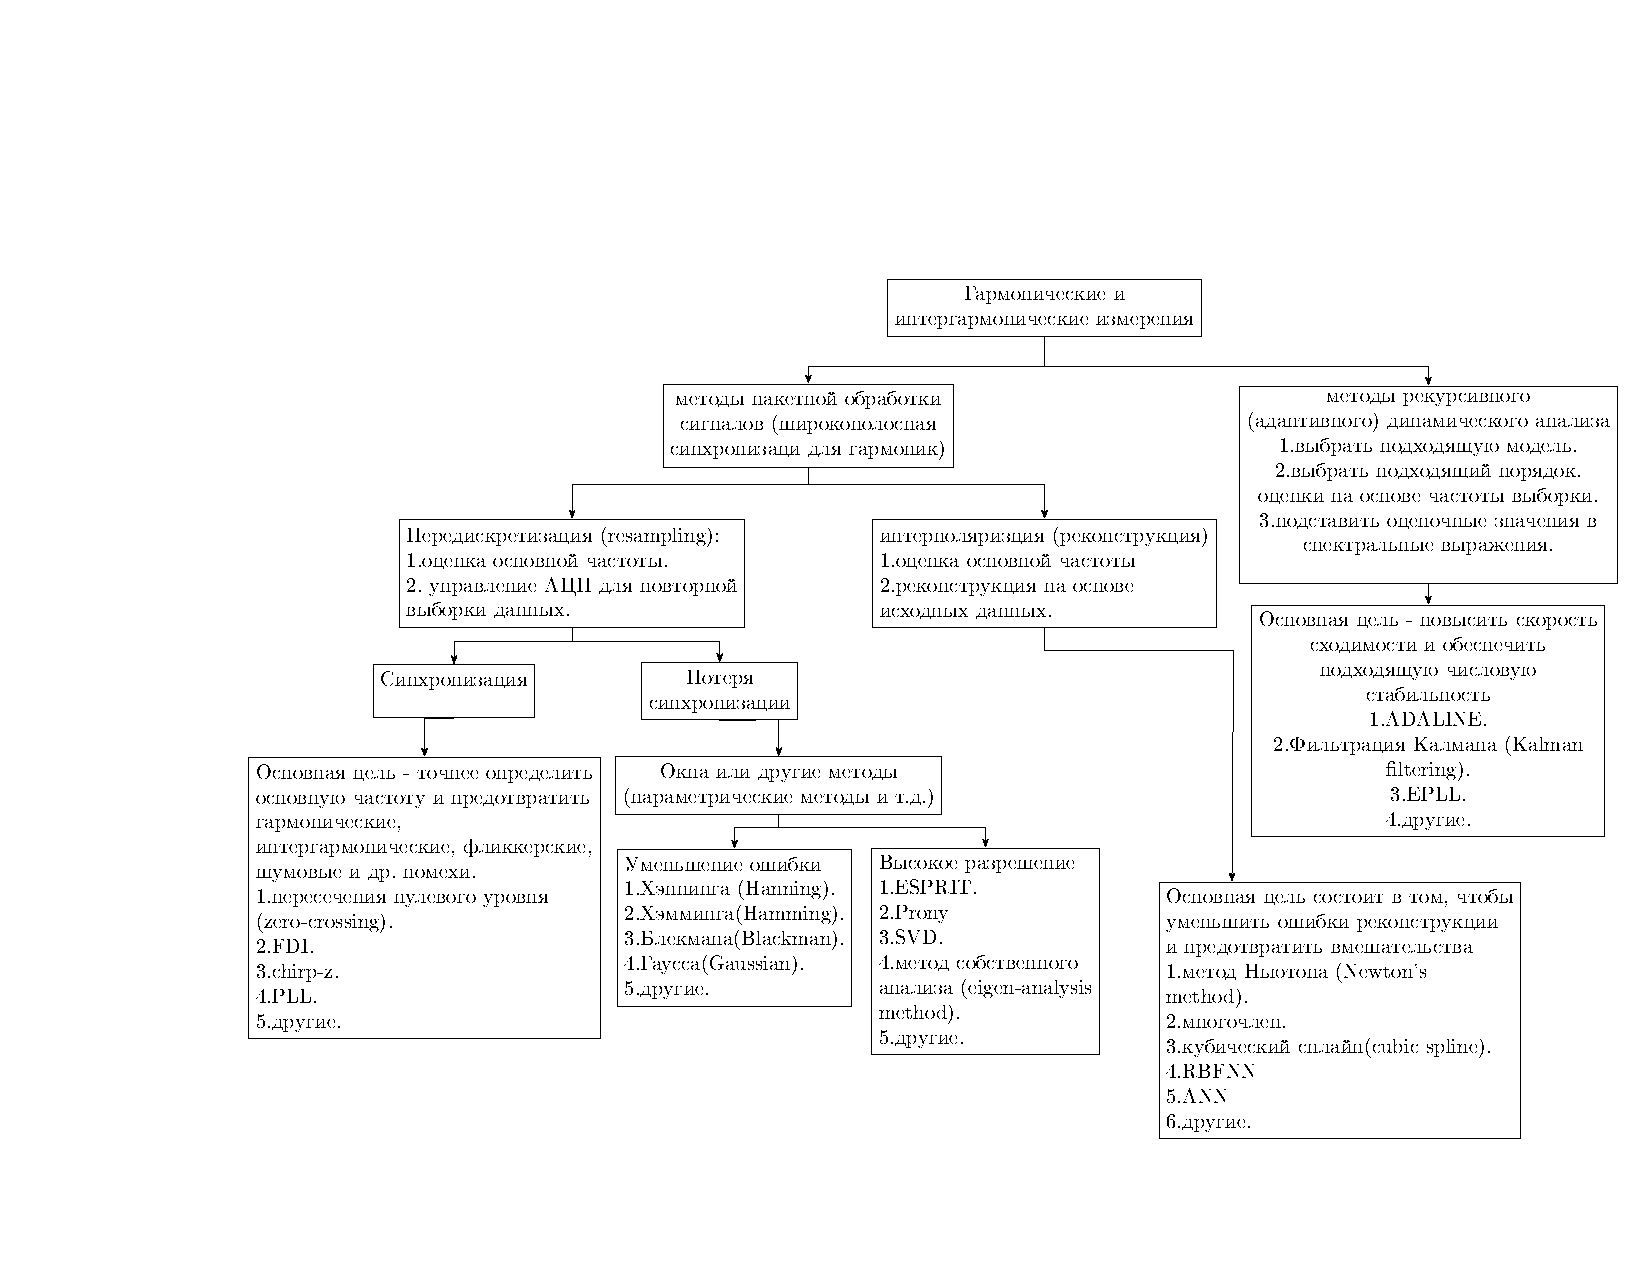
\includegraphics[scale=0.7]{picture15}
	}
	\caption{Упрощенная классификация обычно используемых методов гармонических и межгармонических оценок.}\label{fig:picture1.3}
\end{figure}
\section{Нижняя граница Крамера-Рао} \label{sec:ch1/sec4}

Для определения точности полученных результатов алгоритмы можно проверить с помощью неравенства Крамера-Рао. В зарубежной литературе чаще встречается термин Cramer-Rao lower bound (CRLB), что обозначает <<нижняя граница Крамера-Рао>>. 

В неравенстве Крамера-Рао сигнал имеет наибольшую величину дисперсии при некоторых условиях. Если неравенство Крамера-Рао преобразуется в равенство, то оценка параметров считается наилучшей. Отсюда следует, что дисперсия данной оценки самая маленькая из возможных. Таким образом, данная оценка лучше всех остальных, и метод с такой дисперсией обладает наилучшей точностью \cite{4515960, 343082, kay1993fundamentals, 1439205, 668800, tran1990cramer}.

% S. Bay, B. Geller, A. Renaux, J. Barbot and J. Brossier, "On the Hybrid Cramér Rao Bound and Its Application to Dynamical Phase Estimation," in IEEE Signal Processing Letters, vol. 15, pp. 453-456, 2008, doi: 10.1109/LSP.2008.921461.

% J. A. Fessler and A. O. Hero, "Cramer-Rao lower bounds for biased image reconstruction," Proceedings of 36th Midwest Symposium on Circuits and Systems, Detroit, MI, USA, 1993, pp. 253-256 vol.1, doi: 10.1109/MWSCAS.1993.343082.

% Kay S. M. Fundamentals of statistical signal processing. – Prentice Hall PTR, 1993.

% N. Noels, H. Steendam and M. Moeneclaey, "On the Cramer-Rao lower bound and the performance of synchronizers for (turbo) encoded systems," IEEE 5th Workshop on Signal Processing Advances in Wireless Communications, 2004., Lisbon, Portugal, 2004, pp. 69-73, doi: 10.1109/SPAWC.2004.1439205.

% P. Tichavsky, C. H. Muravchik and A. Nehorai, "Posterior Cramer-Rao bounds for discrete-time nonlinear filtering," in IEEE Transactions on Signal Processing, vol. 46, no. 5, pp. 1386-1396, May 1998, doi: 10.1109/78.668800.

% Tran C. V. Cramer-Rao Bound, MUSIC, and Maximum Likelihood. Effects of Temporal Phase Difference. – NAVAL OCEAN SYSTEMS CENTER SAN DIEGO CA, 1990.

Несмещенная оценка, которая достигается нижней границей Крамера-Рао, называется эффективной. Такое решение обеспечивает наименьшую среднеквадратичную ошибку среди несмещенных методов и называется minimum variance unbiased (MVU)~--~<<оценкой с минимальной несмещенной дисперсией>>.

Информация Фишера играет важную роль в статическом моделировании для построения гипотез с использованием оценок максимального правдоподобия. Функция правдоподобия называется maximum likelihood estimation (MLE), то есть «оценкой максимального правдоподобия». Если можно найти производную из функции правдоподобия, то решение первого порядка производной функции возможно с помощью метода наименьших квадратов. Чаще используют методы определения локальных максимумов и минимумов с помощью численных методов.

\begin{equation}
	\label{eq:equation1.4.1}
	\sigma^2 = 10^{- \frac{SNR}{10}}
\end{equation}

Для амплитуды, частоты и фазы гармоник напряжения неравенство Крамера-Рао выглядит следующим образом \cite{kay1993fundamentals}:

\begin{equation}
	\label{eq:equation1.4.2}
	D(A) \geqslant \frac{2 \sigma^2}{N}
\end{equation}
где $\sigma^2$ --\textbf{дисперсия};

$N$ -- число отчетов БПФ;

$A$ -- амплитуда гармоники.

\begin{equation}
	\label{eq:equation1.4.3}
	D(f) \geqslant \frac{12 \cdot \sigma^2}{A^2 \cdot \pi^2 \cdot N(N-1)(2N-1)}
\end{equation}
где $f$ -- частота гармоник.

\begin{equation}
	\label{eq:equation1.4.4}
	D(\varphi) \geqslant \frac{2 \cdot \sigma^2}{A^2 \cdot \pi^2 \cdot N(N-1)}
\end{equation} 
где $\varphi$ -- фаза гармоник.


В общем случае граница Крамера-Рао определяется следующим образом:
\begin{equation}
	\label{eq:equation1.4.5}
	var(\theta)\geq\frac{1}{-E\left[\frac{(\delta^2 ln p(x;\theta)}{\delta\theta^2}\right]}
\end{equation}

\begin{table} [htbp]
	\centering
	\changecaptionwidth\captionwidth{16cm}
	\caption{Название таблицы}\label{tab:Ts}%
	\begin{tabular}{| p{4cm} || p{6cm} | p{6cm} |}
		\hline
		\hline
		Название & Действительные значения & Комплексные значения \\
		\hline
		Случайные переменные & X & $\widetilde{X}=U+jV (U and V independent)$ \\
		\hline
		Значение & $E{[}x{]} = \int xp(x)dx$ & $E[\widetilde{X}]=\int up_U (u)du+j\int up_V(\upsilon)d\upsilon$ \\
		\hline 
		Дисперсия &  
		$var(X)=E[(X-E[X]^2) \linebreak =\int(x-E[x])^2px(x)dx$   & 
		$var(\widetilde{X})=E[|\widetilde{X}-E[\widetilde{X}]|^2]  =\int |\widetilde{x}-E[\widetilde{X}]|^2pU,V(u,\upsilon)dud\upsilon$ \\
		\hline
		Нормальное распределение &
		$px(x)=\frac{1}{\sqrt{2\pi\sigma^2}} exp [-\frac{1}{2\sigma^2}(x-\mu)^2]$  
		& $p\widetilde{x}(\widetilde{x})=\frac{1}{\sqrt{2\pi\sigma^2}} exp [-\frac{1}{2\sigma^2}|\widetilde{x}-\widetilde{\mu}|^2]$	\\
		\hline
		Свертка & $cov(X,Y)=E[(X-E[X])(Y-E[Y])]$  
		& $cov(X,Y)=E[(\widetilde{X}-E[\widetilde{X}])(\widetilde{Y}-E[\widetilde{Y}])]$ \\
		\hline
		Произвольный вектор &$X=[X_1X_2...X_L]^T$            
		&$X=[\widetilde{X}_1\widetilde{X}_2...\widetilde{X}_L]^T$ \\
		\hline
		Среднее значение вектора &$E[X]=[E[X_1]E[X_2]...E[X_L]]^T$ 
		&$E[\widetilde{X}]=[E[\widetilde{X}_1]E[\widetilde{X}_2]...E[\widetilde{X}_L]]^T$ 
		\\
		\hline
		Матрица свертки  &$C_x=E[(X-E[X])(X-E[X])^T]$ $(C_x^T =C_x)$    
		&$C_x=E[(X-E[X])(X-E[X])^H]$ $(C_x^H =C_x)$ \\
		\hline
		Многомерное нормальное распределение &$px(x)=\frac{1}{(2\pi)^(L/2) det^(1/2)(C_x)}$ $.exp[\frac{1}{2}(x-\mu)^T C_x^(-1)(x-\mu)]$  
		&$p\widetilde{x}(\widetilde{x})=\frac{1}{(\pi)^L det(C_x)}$ 
		\linebreak
		$.exp[-(\widetilde{x}-\widetilde{\mu})^H C_x^(-1)(\widetilde{x}-\widetilde{\mu})]$ \\
		\hline
		Автокорреляция &$r_x[k]=E[x[n]x[n+k]]$        
		&  $r_x[k]=E[x^*[n]x[n+k]]$ \\
		\hline
		Cпектральная плотность мощности & $P_x(f)=\Sigma_k^\infty=\infty r_x[k](-j2\pi fk)$  
		$(P(-f)=P_x(f))$               
		& $P_x(f)=\Sigma_k^\infty=\infty r_x[k](-j2\pi fk)$ \\
		\hline
		Аддитивный белый гауссовский шум & $w{[}n{]}$                       
		&$\widetilde{w}[n]=u[n]+j\upsilon[n]  
		(u[n),\upsilon[n]$ \linebreak) \\
		\hline
		Авторегрессионный метод &
		$x[n]=-\Sigma_k^p a[k]x[n-k]+u[n] (u[n] is WGN)$
		& $\widetilde{x}[n]=-\Sigma_k^p a[k]\widetilde{x}[n-k]+\widetilde{u}[n]$  \linebreak  
		($a[k]^s$ complex and $u[n]$ is CWGN) \\
		\hline
		\hline
	\end{tabular}
\end{table}



\section{Модель сигнала электрической сети} \label{sec:ch1/sec5}
% МОДЕЛЬ СИГНАЛА ЭЛЕКТРИЧЕСКОЙ СЕТИ ДЛЯ ИЗМЕРЕНИЯ ГАРМОНИК И ИНТЕРГАРМОНИК

Гармоника -- это спектральная составляющая на частотах, которая кратна основной частоте системы переменного тока. 

Интергармоника -- это спектральная компонента на частотах, которая зависит от единиц измерения и не кратна основной частоте системы.
Основополагающим нормативным документом в РФ, регламентирующим отличие между гармониками и интергармониками, является государственный стандарт \cite{GOST30804.4.7-2013}. 
%ГОСТ 30804.4.7-2013 (IEC 61000-4-7:2009) Совместимость технических средств электромагнитная. Общее руководство по средствам измерений и измерениям гармоник и интергармоник для систем электроснабжения и подключаемых к ним технических средств. 2013; Доступно по: http://docs.cntd.ru/document/1200103652 

Стандарт  описывает спектральные составляющие тока и напряжения, расположенных выше области частот гармоник $2-9$ кГц. Определение терминов «гармоника» и «интергармоника» в стандарте \cite{GOST30804.4.7-2013}, в разделах $3.2.3$ и $3.4.2$.

Согласно стандарту \cite{GOST32144-2013}, раздел $3.1.19$, под «напряжением интергармонической составляющей» понимают среднеквадратическое значение синусоидального напряжение, частота которого не кратна основной частоте напряжения электропитания.
%ГОСТ 32144-2013 Электрическая энергия. Совместимость технических средств электромагнитная. Нормы качества электрической энергии в системах электроснабжения общего назначения. 2013; Доступно по: http://docs.cntd.ru/document/1200104301 
Если одновременно возникнут интергармонические составляющие на приближенных частотах, то образуется напряжение с широкополосным спектром. В разделе $4.2.4.2$ настоящего стандарта описано, что «допустимые уровни интергармонических составляющих напряжения электропитания находятся на рассмотрении».

В международной электротехнической комиссии (МЭК, IEC -- International Electrotechnical Commission) стандартизация в области интергамоник находится на рассмотрении и накоплении информации. В стандарте [3] интергармоники напряжения ограничиваются значением $0,2\%$.
%3. International Electrotechnical Commission et al. Electromagnetic Compatibility (EMC)-Part 4-7: Testing and Measurement Techniques-General Lighting Res. Technol. 2013; 45: 710–728 Guide on Harmonics and Interharmonics Measurements and Instrumentation, for Power Supply Systems and Equipment Connected Thereto. – IEC 61000-4. – Т. 7.

Кроме Российских стандартов, существуют международные регламентирующие документы по мониторингу качества электроэнергии (КЭ), рекомендация от Института инженеров электротехники (IEEE – Institute of Electrical and Electronics Engineers). Термин гармоника в \cite{6826459} обозначают как «total harmonic distortion (THD)».
% 4. IEEE Recommended Practice and Requirements for Harmonic Control in Electric Power Systems, in IEEE Std 519-2014 (Revision of IEEE Std 519-1992), vol., no., pp.1-29, 11 June 2014, doi: 10.1109/IEEESTD.2014.6826459. Доступно по: https://ieeexplore.ieee.org/servlet/opac?punumber=6826457 (дата обращения: 01.10.2020).
То есть отношение среднеквадратичного значения гармонического содержимого с учетом гармонических составляющих до $50$-го порядка, исключая интергармоники. Пороговые значения интергармоник в сетях низшего (до $1$ кВ), среднего ($69-161$ кВ) и высшего (более $161$ кВ) напряжения.

Наличие интергармоник и гармоник оказывает негативное влияние на оборудование. Из-за возникновения гармоник в электрических сетях происходит перегрев оборудования, поэтому уменьшается его срок службы. Интергармоники наблюдаются при увеличении количества нагрузок в дополнение к гармоникам. Наличие асинхронных включений частотно-регулируемых электроприводов, выполненных на основе полупроводниковых преобразователей является причиной появления интергармоник. Так же интергамоники возникают при изменении тока в оборудовании, которое приводит к колебаниям напряжения. 

Источниками интергармоник в электрических сетях являются асинхронные включения частотно-регулируемых электроприводов, дуговые печи, частотно регулируемые электроприводы. 

Возникновение интергармоник обусловлено модуляцией несинусоидальных процессов, кривые которых содержат только кратные высшие гармоники, а также низкочастотные колебания, характерные для сетей с резко переменными нагрузками. Например, электродуговые сталеплавильные печи, сварочные установки, тиристорные электроприводы \cite{Interharmonics_in_systems_Zhezhelenko_1999}. В зависимости от амплитуды токов высших гармоник возникают искажения напряжения в узлах нагрузок на данной частоте. Повышается вероятность возникновения резонанса, в зависимости от ширины спектра частот интергармоник. 
%5. Жежеленко И. В., Саенко Ю. Л., Бараненко Т. К. Интергармоники в системах электроснабжения промпредприятий //Вестник Приазовского государственного технического университета. Серия: Технические науки. 1999;8. Доступно по: https://cyberleninka.ru/article/n/intergarmoniki-v-sistemah-elektrosnabzheniya-prompredpriyatiy 

В состав промышленных предприятий входят частотно-регулируемые электроприводы. Известно, что данные установки являются характерным источником высших гармоник и генерируют гармоники $5,7,11,13$ и другие. Эти гармоники также генерируются сварочными выпрямителями \cite{Calculation_Current_Mikheev_2017}. Высшие гармоники также называют каноническими гармониками.

%Михеев Г. М. и др. Расчет тока конденсаторных батарей с учетом источников высших гармоник //Вестник Чувашского университета. 2017; 1. Доступно по: https://cyberleninka.ru/article/n/raschyot-toka-kondensatornyh-batarey-s-uchetom-istochnikov-vysshih-garmonik
Проблема измерения гармоник и интергармоник в электрической сети является актуальной. \cite{testa2007интергармоники, gunther2001interharmonics, 532851, testa2002interharmonic}

%7. A. Testa et al., «Interharmonics: Theory and Modeling,» in IEEE Transactions on Power Delivery, vol. 22, no. 4, pp. 2335-2348, Oct. 2007, doi: 10.1109/TPWRD.2007.905505. Доступно по: https://ieeexplore.ieee.org/document/4302786/references#references (дата обращения: 01.10.2020).
%8. E. W. Gunther, «Interharmonics in power systems» 2001 Power Engineering Society Summer Meeting. Conference Proceedings (Cat. No.01CH37262), Vancouver, BC, Canada, 2001, pp. 813-817 vol.2, doi: 10.1109/PESS.2001.970156. Доступно по: https://ieeexplore.ieee.org/document/970156 (дата обращения: 01.10.2020).
%9. R. Yacamini, «Power system harmonics. IV. Interharmonics» in Power Engineering Journal, vol. 10, no. 4, pp. 185-193, Aug. 1996, doi: 10.1049/pe:19960411. https://ieeexplore.ieee.org/document/532851  Доступно по:  (дата обращения: 01.10.2020).
%10. Gallo D., Langella R., Testa A. Interharmonic measurement in IEC framework //IEEE Summer Power Meeting. 2002. Доступно по: https://iris.unicampania.it/handle/11591/206785#.XoBAHogzZPY (дата обращения: 01.10.2020).
 
Спектральный анализ гармоник и интергармоник так же представлен в отечественных работах. \cite{Improving_methods_Shizma_2014,Harmonic_analysis_Goldstein2009, Development_method_Osipov_2017}

%11.Чижма С. Н. Совершенствование методов и средств контроля качества электроэнергии и составляющих мощности в электроэнергетических системах с тяговой нагрузкой //Омск: Омский государственный университет путей сообщения. 2014; Доступно по: https://omgtu.ru/scientific_activities/dissertatsionnye_sovety/obyavleniya_o_zashchite_dissertatsiy_i_dokumenty_k_nim/chizhma_s_n/ (дата обращения: 01.10.2020).
%12.  Гольдштейн Е. И., Радаев Е. В. Гармонический анализ токов (напряжений) при наличии в них интергармоник и неизвестном периоде результирующего сигнала //Электричество. – 2009. – №. 12. – С. 87-88.
%13. Осипов Д. С. и др. Разработка метода расчета потерь мощности в токоведущих частях при наличии интергармоник //Омский научный вестник. – 2017. – №. 4 (154). 


В \cite{Improving_methods_Shizma_2014} рассмотрен метод канонических гармоник и интергармоник. Реализация с помощью оконного преобразования Фурье (ОПФ) с применением оконных функций низкого разрешения и интерполяции. 
%11.Чижма С. Н. Совершенствование методов и средств контроля качества электроэнергии и составляющих мощности в электроэнергетических системах с тяговой нагрузкой //Омск: Омский государственный университет путей сообщения. 2014; Доступно по: https://omgtu.ru/scientific_activities/dissertatsionnye_sovety/obyavleniya_o_zashchite_dissertatsiy_i_dokumenty_k_nim/chizhma_s_n/ (дата обращения: 01.10.2020).


Авторы \cite{Harmonic_analysis_Goldstein2009} работы перед проведением дискретного преобразования Фурье (ПФ) предложили догармонический анализ сигнала. Т.е. предварительное определение частот, входящих в исходный сигнал путем расчета среднеквадратичного отклонения, определение периода сигнала электрической сети путем нахождения общего делителя. 
%12.  Гольдштейн Е. И., Радаев Е. В. Гармонический анализ токов (напряжений) при наличии в них интергармоник и неизвестном периоде результирующего сигнала //Электричество. – 2009. – №. 12. – С. 87-88.


В \cite{Development_method_Osipov_2017} разработан алгоритм расчета дополнительных потерь в токоведущих частях при наличии интергармоник, генерируемых частотно-регулируемым приводом на основе пакетного вейвлет-преобразования (ПВП).
%13. Осипов Д. С. и др. Разработка метода расчета потерь мощности в токоведущих частях при наличии интергармоник //Омский научный вестник. – 2017. – №. 4 (154). 

Спектральные составляющие на частотах, расположенных между двух последовательных гармонических частот, возникают при наличии в сигнале интергармонических составляющих. 
Заметные интергармоники появляются в узком диапазоне частот: $35$ – $75$ Гц, $150$ – $160$ Гц \cite{Interharmonics_in_systems_Zhezhelenko_1999}.
% Жежеленко И. В., Саенко Ю. Л., Бараненко Т. К. Интергармоники в системах электроснабжения промпредприятий //Вестник Приазовского государственного технического университета. Серия: Технические науки. 1999;8. Доступно по: https://cyberleninka.ru/article/n/intergarmoniki-v-sistemah-elektrosnabzheniya-prompredpriyatiy 
 
Модель сигнала электрической сети с учетом \cite{GOST30804.4.7-2013}, раздел $3.1$, связывает гармоники, высшие гармоники и интергармоники тока и напряжения электрической сети при наличии шума: 
%ГОСТ 30804.4.7-2013 (IEC 61000-4-7:2009) Совместимость технических средств электромагнитная. Общее руководство по средствам измерений и измерениям гармоник и интергармоник для систем электроснабжения и подключаемых к ним технических средств. 2013; Доступно по: http://docs.cntd.ru/document/1200103652
\begin{equation}
	\label{eq:equation6}
		s_{t} = a_{0} \sin (\omega_{0} t + \varphi_{0}) + \displaystyle\sum_{p=0}^{p} a_p^{\upsilon} \sin (m_p^{\upsilon} \omega_{0} t + \varphi_p^{\upsilon}) + \displaystyle\sum_{q=0}^{q} a_q^i \sin  (\omega_q^i t + \varphi_q^{i})
\end{equation}

где $a_{0}$ – амплитуда первой гармоники;

$\omega_{0}$ – угловая частота первой гармоники, $\omega_{1} = 2 \pi f_{H,1}$;

$\varphi_{0}$ – фаза первой гармоники; 

$p$ – число высших гармоник;

$a_p^{\upsilon}$ – амплитуда высших гармоник;

$m_p^{\upsilon}$ – номер высших гармоник;

$\varphi_p^{\upsilon}$ – фаза высших гармоник;

$q$– номер интергармоник;

$a_q^i$ – амплитуда интергармоник;

$\omega_q^i$ – угловая частота интергармоник, $\omega_q^i=2\pi f_{ig,h}$; 

$f_{ig,h}$ – частота интергармонической подгруппы порядка $h$;

$\eta$ – шум.

В формулу \ref{eq:equation6} добавлены значения высших гармоник, интергармоник тока и напряжения электрической сети.
Согласно \cite{GOST32144-2013}, раздел $4.2.4$, к показателям качества электрической энергии (КЭ), относятся гармонические составляющие напряжения, т.~е. коэффициент  $n$ гармонической составляющей напряжения – $K_{U(n)}$:
%ГОСТ 32144-2013 Электрическая энергия. Совместимость технических средств электромагнитная. Нормы качества электрической энергии в системах электроснабжения общего назначения. 2013; Доступно по: http://docs.cntd.ru/document/1200104301 

\begin{equation}
	\label{eq:equation7}
K_{U(n)} = \frac{U_{(n)}}{U_1}
\end{equation}

где $n$ – номер гармонической составляющей напряжения;
 
$U_{(n)}$ – фазное напряжение гармоники в расчетной точке сети, В,кВ;

$U_1$ – значение основной гармонической составляющей напряжения, В,кВ.

\begin{equation}
	\label{eq:equation8}
	U_(n) = \frac{I_{(n)} n U_{nl} U_{nom}}{S_k}
\end{equation}

где n – номер гармонической составляющей напряжения;

$I_{(n)}$ – действующее значение фазного тока -ой гармоники, А,кА;

$U_{nl}$ – напряжение нелинейной нагрузки (в случае, если расчетная точка совпадает с точкой присоединения нелинейной нагрузки $U_{nl} = U_{nom}$, В,кВ;

$U_{nom}$ – номинальное напряжение сети, В,кВ;

$S_k$ – мощность короткого замыкания в точке присоединения нелинейной нагрузки, кВ А.

Значения коэффициентов нечетных гармонических составляющих напряжения не кратных трем $K_{U(n)}=0,4$ \% $U_1$ для $n>25$, при напряжении электрической сети $110-220$ кВ.

Значения коэффициентов нечетных гармонических составляющих напряжения кратных трем $K_{U(n)}=0,2$ \% $U_1$ для $n>21$, при напряжении электрической сети $110-220$ кВ.

Значения коэффициентов четных гармонических составляющих напряжения $K_{U(n)}=0,2$ \% $U_1$ для $n>21$, при напряжении электрической сети $110-220$ кВ.
Согласно \cite{GOST32144-2013}, раздел $4.2.4$, «Допустимые уровни интергармонических составляющих напряжения электропитания находятся на рассмотрении».
%2. ГОСТ 32144-2013 Электрическая энергия. Совместимость технических средств электромагнитная. Нормы качества электрической энергии в системах электроснабжения общего назначения. 2013; Доступно по: http://docs.cntd.ru/document/1200104301

Абсолютное значение амплитуды интергармоник $a_q^i$ изменяется в диапазоне $0,4-1$ для частоты $60$ Гц и $90$ Гц \cite{testa2007интергармоники}.
%7. A. Testa et al., «Interharmonics: Theory and Modeling,» in IEEE Transactions on Power Delivery, vol. 22, no. 4, pp. 2335-2348, Oct. 2007, doi: 10.1109/TPWRD.2007.905505. Доступно по: https://ieeexplore.ieee.org/document/4302786/references#references

В \cite{Improving_methods_Shizma_2014, ramos2017power}описаны принципы построения многофункциональных измерительных комплексов для электроподвижного состава и тяговых подстанций.
% 11. Чижма С. Н. Совершенствование методов и средств контроля качества электроэнергии и составляющих мощности в электроэнергетических системах с тяговой нагрузкой //Омск: Омский государственный университет путей сообщения. 2014; Доступно по: https://omgtu.ru/scientific_activities/dissertatsionnye_sovety/obyavleniya_o_zashchite_dissertatsiy_i_dokumenty_k_nim/chizhma_s_n/
% 14. Ramos C. J., Martins A. P., da Silva Carvalho A. Power system frequency estimation using a least mean squares differentiator //International Journal of Electrical Power & Energy Systems. 2017;87:166-175. Доступно по: https://www.sciencedirect.com/science/article/abs/pii/S0142061516315587. DOI: 10.1016/j.ijepes.2016.11.001
Наличие высокочастотных составляющих в сигналах токов и напряжений, определяют кривые первичных токов и напряжений электровоза с помощью прибора ИВК «Омск-М». Испытания проводились в Абаканской дистанции электроснабжения Красноярской дирекции по энергообеспечению. Анализ гармонических составляющих для спектра гармоник напряжений показал, что процент от амплитуды $1$-й гармоники от $5$ гармоники, будет равен $8$. И процент от амплитуды $1$-й гармоники будет равен $100$ на $2$ гармоники для спектра гармоник токов.

Анализ и контроль гармоник сигнала в электрической сети имеет большое значение для поддержания качества электрической энергии, предотвращения повреждения систем электрических сетей и экономии энергии. 

В работе представлена математическая модель сигнала в электрической сети, обобщающая результаты исследований проблем качества электроэнергии и учитывающая требования регламентирующих документов. Она позволяет проводить исследования алгоритмов анализа электрических сигналов, а также средств измерений, построенных на их основе.

\section{Выводы по разделу} \label{sec:ch1/sec6} 

В результате анализа, произведенного в первом разделе, можно сделать следующие выводы:
\begin{itemize}
\item Особенности сигналов в электрических сетях носят не существенный характер с точки зрения построения алгоритмов нахождения параметров гармоник. При работе с электрическими сетями обычно используют стандартные алгоритмы такого рода.

\item Помимо обычных алгоритмов для оценки параметров гармоник в электрических сетях также используют алгоритмы, анализирующие сигналы в переходных режимах, т.е. такие, в которых во время работы алгоритма может измениться значение какого-либо параметра. В нашей работе такие алгоритмы далее рассматриваться не будут, поскольку переходные режимы не являются целью нашей работы.

\item Анализ имеющихся библиографических источников показывает, что нет известных публикаций в которых бы велась разработка алгоритмов, ориентированных на работу при определенном соотношении сигнал-шум, и что для анализа гармоник и интергармоник (для которых это соотношение отличается) применяются одинаковые алгоритмы.

\item Алгоритмы оценки параметров гармоник, применяемые при работе с одно- и многотональными сигналами, имеют точность оценки параметров ниже теоретической границы Крамера-Рао. Вопрос о причинах снижения точности и возможности построения алгоритма, достигающего этой границы в известных научных публикациях не рассмотрен.

\item Для решения задачи построения оптимального алгоритма для анализа спектра сигнала в электрических сетях необходимо уточнение математической модели спектра сигналов в части, описывающей точность оценки (дисперсию) параметров гармоник спектра многотонального сигнала.
\end{itemize}

